
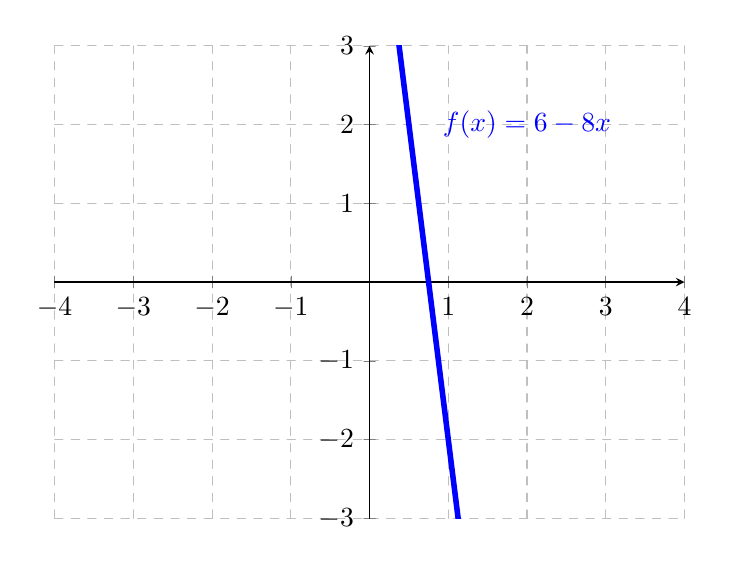
\begin{tikzpicture}[line cap=round,line join=round,>=stealth,x=1cm,y=1cm, scale=1]
\begin{axis}[
x=1cm,y=1cm,
axis lines=middle,
grid style=dashed,
ymajorgrids=true,
xmajorgrids=true,
xmin=-4,    %Valor mínimo que no sobrepasa la gráfica
xmax=4,     %Valor máximo que no sobrepasa la gráfica
ymin=-3,
ymax=3,
xtick={-4,-3,...,4},    % Etiquetas de los ejes
ytick={-3,-2,...,3},]   
\clip(-4,-3) rectangle (4,3);   % Tamaño del rectangulo de los ejes
\draw[line width=2pt,color= blue,smooth,samples=100,domain=-4:4] plot(\x,{6-8*(\x)});    %Función a gráficar
\draw[color= blue] (2,2) node {$f(x) = 6 - 8x$};    % Etiquetar
\end{axis}
\end{tikzpicture}